% statistics_and_probability:x16 GDC:YES
\begin{question}
  \hspace*{\fill} [Note maximale: 7]\par
  \medskip
  \noindent Soit la variable aléatoire X normalement distribuée avec une moyenne de 25,\par
  \noindent comme le montre la figure ci-dessous.\par
  \medskip
  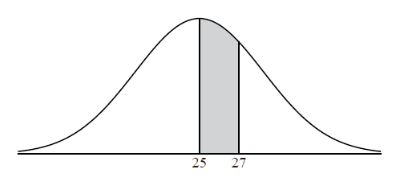
\includegraphics[scale=0.5]{normale_moyenne}\par
  \medskip
  \noindent La région grisée entre 25 et 27 représente 30\% de la distribution.\par
  \medskip
  (a) Trouvez $ P(X > 27) $\hspace*{\fill} [2]\par
  \medskip
  (b) Trouvez l’écart-type de X.\hspace*{\fill} [5]\par

\end{question}

